\chapter{Revisão da literatura}

A seguir será discorrido sobre os aspectos mais relevantes que envolvem a aplicação de soluções de fotopletismografia remota. Ademais, serão apresentados os principais algoritmos e modelos da literatura e suas características. Com essa revisão, espera-se estabelecer o contexto do desenvolvimento deste projeto de forma completa e esclarecedora. 

\section{Modelagem do comportamento óptico da pele}

A implementação de métodos de rPPG é baseada em uma fonte de iluminação, seja ela natural ou artificial, a qual interage com o tecido biológico de modo que a luz re-emitida após essa interação contém o sinal de interesse a partir do qual podem ser extraídos parâmetros fisiológicos. Por isso, o desenvolvimento de algoritmos capazes de processar os dados captados por um dispositivo de aquisição de imagens para obter esse sinal faz necessário o equacionamento de modelos que descrevem os fenômenos ópticos da pele. Nesse sentido, a literatura cita duas principais abordagens, que serão discutidas em seguida. 

\subsection{Lei de Beer-Lambert}
\label{sec:beer-lambert}

A Lei de Beer-Labert é um princípio da espectroscopia que explica como a quantidade de luz atenuada por uma substância depende de sua concentração e do caminho percorrido pelo feixe luminoso. A equação \ref{eq:beer-lambert} descreve essa relação, sendo \(A\) a absorbância em um determinado comprimento de onda \(\lambda\), ou seja, a quantidade de luz absorvida, \(\varepsilon\) a absortividade molar, que caracteriza a intensidade com que uma espécie química absorve luz, \(c\) a concentração da substância e \(l\) o comprimento do caminho percorrido pelo feixe. 

\begin{equation}
\label{eq:beer-lambert}
    A(\lambda) = \varepsilon(\lambda) \cdot c \cdot l(\lambda)
\end{equation}

Assim, o modelo de absorbância da pele pode ser descrito conforme a equação:

\begin{equation}
\label{eq:absorb-beerlamb}
    A(\lambda) = v_m(\lambda)c_m + v_h(\lambda)c_h + A_0(\lambda)
\end{equation}

em que \(v\) representa o produto \(\varepsilon \cdot l\), \(A_0\) denota a absorção basal cutânea, considerando a saturação de oxigênio do sangue arterial constante, e os índices \(h\) e \(m\) representam a contribuição da hemoglobina e da melanina, respectivamente, considerando que essas são as substâncias que influenciam de forma predominante as características da pigmentação da pele. 

A absorbância também pode ser expressa em função da intensidade de luz incidente (\(E\)) e transmitida (\(L\)): 

\begin{equation}
    A = - log_{10}\Big (\frac{L}{E} \Big )
\end{equation}

Descreve-se, então, o modelo de formação da imagem de uma câmera, por meio do modelo da intensidade \( P_i \) de um pixel em uma posição \((x, y)\) de uma imagem correspondente a uma área da pele captada por uma câmera em um canal \(i= \{R, G, B \}\) como:

\begin{equation}
    \label{eq:Pi-beerlambert}
    P_i(x, y) = k \int L(x, y, \lambda) S_i(\lambda) d \lambda
\end{equation}

em que \(S_i\) refere-se à resposta espectral do sensor e \(k\) ao ganho da câmera \cite{xu2014robust}. 

Alternativamente a esse modelo, baseado na luz absorvida em uma posição estática, é possível modelar esse sistema com base na luz refletida ao longo do tempo. Para isso, descreve-se a curva de reflexão da pele em um instante de tempo como:

\begin{equation}
    \label{eq:Rs}
    R_s(\lambda) = a_m R_m(\lambda) + a_h R_h(\lambda)
\end{equation}

em que \(R_s\) descreve a refletância espectral da pele, \(R_m\) e \(R_h\) são as componentes espectrais associadas à melanina e à hemoglobina, respectivamente, e \(a_m\) e \(a_h\) são coeficientes escalares que ponderam a contribuição relativa de cada componente.

A partir disso, modela-se em função do tempo o valor de um pixel da região da pele captado por um canal de cor de uma câmera de acordo com a equação \ref{eq:pixel-beerlambert-reflection} \cite{lam2015robust}.

\begin{equation}
    \label{eq:pixel-beerlambert-reflection}
   C_i(t) = a_m a_I(t) \int R_m(\lambda) I(\lambda, t) S_k(\lambda) d\lambda + a_h(t) a_I(t) \int R_h(\lambda, t) I(\lambda, t) S_i(\lambda) d\lambda
\end{equation}

Nesse caso, \(a_I\) é um fator escalar associado às variações temporais de iluminação, \(I(\lambda, t)\) é o espectro normalizado da fonte luminosa e \(S_i(\lambda)\) é a resposta espectral da câmera para o canal \(i\).

\subsection{Modelo Dicromático de Reflexão}

Paralelamente, em vista dos conceitos da computação gráfica e da visão computacional, a interação da luz com materiais dielétricos, como a pele, é descrita em termos de componentes independentes de reflexão especular e de reflexão difusa \cite{klinker1988measurement}. No contexto da fotopletismografia remota, a primeira refere-se à energia luminosa que não é absorvida pelos tecidos e não possui informações referentes à pulsação. A componente difusa, por sua vez, está associada a absorção e dispersão da luz após atravessar as camadas cutâneas. 

Esse modelo é equacionado de acordo com a relação \ref{eq:dicromatic-general}, em que \(C_k\) é referente a um canal de cor de um pixel \(k\), \(I\) denota a intensidade luminosa, \(v_s\) e \(v_d\) referem-se, respectivamente, às componentes especular e difusa e \(v_n\) denota o ruído de quantização do sensor da câmera. 

\begin{equation}
    \label{eq:dicromatic-general}
    \bm{C_k}(t) = I(t) \cdot (\bm{v_s}(t) + \bm{v_d}(t)) + \bm{v_n}(t)
\end{equation}


No que se refere à componente especular, pode-se expressar \(\bm{v_s}(t)\) segundo a equação \ref{eq:dicromatic-vs}, sendo \(\bm{u_s}\) o vetor unitário de cor do espectro da luz, \(s_0\) a parte estacionária da reflexão especular e \(s(t)\) a parcela variável induzida pelo movimento. 

\begin{equation}
    \label{eq:dicromatic-vs}
    \bm{v_s}(t) = \bm{u_s} \cdot (s_0 + s(t))
\end{equation}

No que se refere à componente difusa,  pode-se descrever \(\bm{v_d}(t)\) segundo a relação \ref{eq:dicromatic-vd}, em que \(\bm{u_d}\) denota o vetor unitário de cor do tecido cutâneo, \(d_0\) é a intensidade de reflexão difusa estacionária, \(\bm{u_p}\) é a intensidade de pulso relativa nos canais RGB e \(p(t)\) é o sinal de pulso \cite{wang2016algorithmic}.

\begin{equation}
    \label{eq:dicromatic-vd}
    \bm{v_d(t)} = \bm{u_d} \cdot d_0 + \bm{u_p} \cdot p(t)
\end{equation}

Visto isso, a modelagem da interação da pele com a luz realizada por meio das diferentes abordagens expostas nas equações \ref{eq:Pi-beerlambert}, \ref{eq:pixel-beerlambert-reflection} e \ref{eq:dicromatic-general} permite o desenvolvimento de algoritmos que extraem o sinal de volume de pulso sanguíneo a partir das variações dos canais RGB captadas por uma câmera ao longo do tempo de uma região do tecido. Para isso, as diferentes abordagens, que serão doravante expostas, utilizam técnicas sobretudo para diminuir as influências dos artefatos de ruído e otimizar fontes específicas do sinal. Por fim, a estimativa de parâmetros fisiológicos pode ser realizada por meio do processamento posterior da forma de onda de BVP obtida.

\section{Métodos não supervisionados}

As primeiras implementações de sistemas de estimação de sinais vitais por fotopletismografia remota que tangem o escopo deste projeto baseiam-se sobretudo em algoritmos e modelos matemáticos cujo objetivo principal é tratar dados de vídeo de câmeras convencionais e extrair o sinal de forma a minimizar o ruído. Para isso, uma das soluções iniciais utilizou uma combinação de métodos de interpolação, derivação de primeira ordem, filtros digitais e análise espectral autorregressiva para processar o nível de intensidade dos pixels de uma ROI definida no rosto de indivíduos gravados por uma câmera com sensor CCD (\textit{Charged-Coupled Device}). Essa análise permitiu a obtenção da frequência cardíaca e da frequência respiratória, as quais demonstraram boa correlação com medições realizadas por um oxímetro de pulso para indicação da frequência cardíaca e com um termistor para detecção de alterações na temperatura no fluxo de ar nasal \cite{takano2007heart}. Outra solução, em contrapartida, realizou uma análise espectral baseada na Transformada Rápida de Fourier (FFT) a partir da média espacial dos pixels de regiões do rosto de indivíduos gravados por uma câmera RGB. Nesse caso, foi possível determinar dados das frequências cardíaca e respiratória, além de propor a hipótese da influência predominante do canal de cor verde sobre o sinal de rPPG  \cite{verkruysse2008remote}. 

\subsection{Métodos baseados em separação de sinais}

Desenvolvimentos subsequentes buscaram procuraram aumentar a separabilidade entre o sinal fisiológico de interesse e componentes associadas a ruído, movimento ou variações de iluminação por meio de técnicas de separação cega de sinais (BSS - \textit{blind source separation}). Esse tipo de abordagem visa a recuperação de sinais-fonte a partir de observações que correspondem a uma mistura dessas fontes. Em BSS, costuma-se partir de um modelo de mistura: \(\bm{C}(t)=\bm{A} \cdot \bm{S}(t) + \bm{n}(t)\), em que \(\bm{C}(t)\) é o vetor de sinais observados, \(\bm{S}(t)\) é o vetor de fontes latentes, \(\bm{A}\) é a matriz de mistura e \(\bm{n}(t)\) representa ruído ou componentes não modeladas. A equação \ref{eq:BSS} enuncia esse conceito, de forma que \(\bm{Y}(t)\) refere-se aos sinais-fonte, \(\bm{C}(t)\) é o sinal observado e \(\bm{W}\) é uma matriz de separação. No contexto da fotopletismografia remota, a fonte é o sinal de pulso de volume sanguíneo e a informação observada corresponde à variação dos canais de cor captada por uma câmera, que contém os artefatos de ruído relacionados a movimento, iluminação, características ópticas da pele e ruído de aquisição.

\begin{equation}
    \label{eq:BSS}
    \bm{Y(t)} = \bm{W} \cdot \bm{C(t)}
\end{equation}

Assim, uma das maneiras de estimar a matriz de separação que permite a obtenção do sinal de interesse é por Análise de Componentes Independentes (ICA) sob a hipótese de independência estatística das fontes. Esse método consiste na recuperação de sinais independentes a partir de observações compostas por combinações lineares das fontes desconhecidas. Especificamente em soluções de rPPG, uma das abordagens utiliza diagonalização conjunta aproximada de matrizes \cite{cardoso1999high} a fim de decompor o sinal normalizado dos canais RGB em três fontes independentes. A partir dessas fontes, é realizada a análise espectral baseada em FFT para obtenção da frequência cardíaca \cite{poh2010non} ou, ainda, de sua variabilidade, bem como da frequência respiratória \cite{poh2010advancements}.  

Outro método baseado em separação de sinais que permite estimar o sinal fisiológico de interesse é por Análise de Componentes Principais (PCA). Essa técnica é tipicamente utilizada para redução de dimensionalidade de conjuntos de dados para reconhecimento estatístico de padrões e processamento de sinais, de modo que determina combinações lineares ortogonais de variáveis originais que maximizam a variância dos dados projetados. No contexto da fotopletismografia remota, a PCA pode ser empregada para decompor os sinais obtidos a partir dos canais de cor em componentes não correlacionadas, podendo evidenciar a componente associada à atividade cardiovascular e, consequentemente, a identificação da frequência cardíaca com custo computacional menor e com desempenho reportado como comparável ao da ICA em determinadas condições experimentais \cite{lewandowska2012measuring}.

\subsection{Métodos baseados em modelos}

Os métodos baseados em BSS são soluções matemáticas e computacionais para processamento de sinais e, no entanto, não incorporam explicitamente as especificidades do comportamento óptico do sinal de rPPG. Por isso, implementações posteriores baseadas em modelos fundamentam-se essencialmente na modelagem de vetores de cor de diferentes componentes para extração das informações de pulso a partir do sinal captado por câmeras RGB. 

Uma dessas implementações é a técnica baseada em crominância \cite{de2013robust}, a qual estipula, a partir do modelo dicromático de reflexão, que artefatos de movimento geram variações na componente de reflexão especular, as quais dependem do ângulo entre a câmera, a pele e a fonte de luz e são aproximadamente idênticas para todos os canais de cor \(R\), \(G\) e \(B\) referentes ao vermelho, verde e azul, respectivamente. Assim, esse algoritmo, daqui em diante referido como CHROM, busca atenuar a influência da componente especular e de perturbações comuns aos três canais, por meio da utilização de dois sinais de crominância ortogonais \(X = R -G\) e \(Y = 0.5 R + 0.5 G - B\), relativos às diferenças entre os sinais de cor, o que pode aumentar a robustez da extração frente a perturbações comuns aos canais de cor. Essa abordagem estabelece, ademais, uma direção de cor de pele padronizada no espaço RGB normalizado, obtida empiricamente, assumindo que a cor média da pele, após normalização, apresenta uma orientação relativamente estável sob iluminação branca. Essa hipótese, exposta na equação \ref{eq:chrom}, permite construir projeções de crominância menos sensíveis à intensidade luminosa, mas não elimina completamente a dependência em relação ao espectro da iluminação, à câmera e às características individuais da pele.

\begin{equation}
\label{eq:chrom}
    S = X_f - \alpha Y_f \quad com \quad \alpha =  \frac{\sigma(X_f)}{\sigma(Y_f)}
\end{equation}

Nessa relação, \(S\) é a estimativa do sinal de pulso, \(X_f\) e \(Y_f\) são os sinais de crominância normalizados em função do vetor padrão de cor de pele \(X_s\) e \(Y_s\) filtrados por um filtro passa-banda, \( \sigma(\cdot) \) é o operador de desvio padrão e \( \alpha \) é um fator de correção que mantém os sinais \(X \) e \(Y \) com amplitudes similares de forma que o ruído especular possa ser efetivamente eliminado. Mais especificamente, define-se:

\begin{equation}
\begin{aligned} 
    X_s &= 3 R_n - 2 G_n \\
    Y_s &= 1.5 R_n + G_n - 1.5 B_n
\end{aligned}
\end{equation}

onde \(R_n\), \(G_n\) e \(B_n\) são os canais referentes ao vermelho, verde e azul, respectivamente. normalizados pelas médias correspondentes.

Outro método, denominado PBV \cite{de2014improved}, baseia-se na análise de que os diferentes espectros de absorção do sangue arterial e do tecido cutâneo causam variações em um vetor característico no espaço RGB normalizado. A partir disso, a definição desse vetor padrão de pulso de volume sanguíneo,\(\ \vec{P_{bv}}\), reflete as amplitudes relativas do sinal de pulso nos canais de cor e depende do espectro de iluminação, da reflectância da pele e dos filtros ópticos da câmera, conforme as equações \ref{eq:pbv-vec} e \ref{eq:pbv-pc}, em que \( \lambda \) é o comprimento de onda, \( H_c \) é a resposta de um canal \(c\) da câmera RGB, \( \rho_s \) é a reflectância da pele, \( I(\lambda) \) é a composição espectral da fonte de luz e \( I_h(\lambda) \) é o espectro contínuo de emissão da lâmpada de halogênio utilizada para medir a amplitude \( PPG(\lambda) \) do sinal de rPPG.

\begin{equation}
    \label{eq:pbv-vec}
    \vec{P_{pbv}}  = [ P_c], \:  c \in \{ R, G, B \}
\end{equation}

\begin{equation}
\label{eq:pbv-pc}
     P_{c} =  \frac{ \int_{400}^{700} H_c(\lambda) \cdot \frac{I(\lambda)}{I_h(\lambda)} \cdot PPG(\lambda) \cdot d \lambda }{ \int_{400}^{700} H_c(\lambda) \cdot \frac{I(\lambda)}{I_h(\lambda)} \cdot \rho_s(\lambda) \cdot d \lambda } 
\end{equation}

Assim, o algoritmo busca encontrar pesos \( \vec{W}_{PBV}\) que fazem com que o sinal \(\vec{S}\) tenha correlação com os canais de cor normalizados \(C_n \in  \{\vec{R_n}, \vec{G_n},  \vec{B_n} \} \) de forma proporcional ao vetor definido, conforme a equação \ref{eq:pbv-general}. 

\begin{equation}
    \label{eq:pbv-general}
    \vec{S} \: C_n^T = k \vec{P_{bv}} \Leftrightarrow \vec{W}_{PBV} C_n C_n^T = k \vec{P_{bv}}
\end{equation}

A técnica de rotação de subespaço espacial (\textit{Spatial Subspace Rotation}, 2SR) \cite{wang2015novel}, por sua vez, define um subespaço que considera a distribuição dos pixels relativos à pele no espaço RGB de modo específico à cada dado de vídeo. Dessa forma, temporalmente, as mudanças nos canais de cor causadas pela pulsação sanguínea geram variações de rotação nesse subespaço. O sucesso desse algoritmo, no entanto, depende de uma máscara bem definida da região da face.  

De forma análoga, o modelo de plano ortogonal à pele (\textit{Projection Orthogonal to Skin}, POS) \cite{wang2016algorithmic} propõe um plano de projeção ortogonal ao vetor de tom de pele no espaço RGB normalizado temporalmente, no qual supõe-se que as componentes especular e difusa possuem distribuições distintas e podem, portanto, ser desagregadas. A equação \ref{eq:pos-s} expõe a relação desse plano, cuja matriz de projeção é denominada \(\bm{P_P}\), para a obtenção do sinal de pulso \(\bm{S}(t)\) a partir dos canais de cor normalizados \( \bm{C_n}(t) = \{R_n(t), G_n(t), B_n(t)\} \).

\begin{equation}
\label{eq:pos-s}
    \bm{S}(t) = \bm{P_P} \cdot \bm{C_n}(t)
\end{equation}

Assim, a projeção dos canais sobre os eixos ortogonais de \(\bm{P_P}\) resulta em dois sinais \(S_1\) e \(S_2\) que contêm o comportamento pulsátil do sinal e são definidos em função da amplitude dos canais de cor, sendo que, para uma única fonte, considera-se que a pulsatilidade dos tecidos cutâneos é observada de forma mais acentuada no canal verde, seguido do azul e é menos evidente no canal vermelho, sob condições usuais de iluminação e aquisição com câmeras RGB. Consequentemente, pode-se escrever esses eixos conforme a equação \ref{eq:pos-s1s2}.

\begin{equation}
\label{eq:pos-s1s2}
S(t) =
\begin{pmatrix}
S_1(t) \\
S_2(t)
\end{pmatrix}
\quad \text{com} \quad
\begin{cases}
S_1(t) = G_n(t) - B_n(t) \\
S_2(t) = G_n(t) + B_n(t) - 2R_n(t)
\end{cases}
\end{equation}

Similarmente ao CHROM, esse algoritmo utiliza um fator de correção \(\alpha\) para ajustar a escala relativa entre as duas componentes projetadas \(S_1\) e \(S_2\), de forma que a obtenção do sinal de rPPG \(h(t)\) é, então, obtida pela combinação linear dessas componentes, conforme exposto pela equação \ref{eq:pos-tuned}.

\begin{equation}
\label{eq:pos-tuned}
    h(t) = S_1(t) + \alpha \cdot S_2(t) \quad com \quad \alpha = \frac{\sigma(S_1)}{\sigma(S_2)}
\end{equation}

Em contraste, o método de invariância local a grupo (\textit{Local Group Invariance}, LGI) \cite{pilz2018local} propõe a construção de uma representação de características invariante a transformações locais, como movimento facial e variações de iluminação. Para isso, modela-se o sinal RGB como um processo aleatório multivariado e utiliza-se a matriz de covariância das transformações para identificar direções de maior variabilidade associadas a fatores de interferência. A partir de uma decomposição espectral, projeta-se o sinal no subespaço ortogonal a essas direções, obtendo-se uma representação mais robusta ao ruído. Em seguida, o sinal transformado é modelado como um processo oscilatório estocástico, capaz de capturar a natureza quase-periódica e não estacionária da frequência cardíaca, por meio do qual esse parâmetro pode ser estimado. 

Complementarmente, o algoritmo de transformação de imagem por matriz ortogonal (\textit{Orthogonal Matrix Image Transformation}, OMIT) \cite{casado2023face2ppg} gera sinais RGB não correlacionados por meio de decomposição QR. Para isso, toma-se a matriz dos canais de cor, uma base ortonormal e uma matriz triangular que contém coeficientes para expressar as colunas da matriz dos canais como uma combinação linear dos vetores da base. Assim, a matriz da base é utilizada para obter uma matriz de projeção que permite a extração da onda de pulso de volume sanguíneo a partir dos dados de cor de entrada. Em adição, esse estudo introduz um fluxo de processamento que inclui uma malha de detecção de pontos da face a qual permite a consistência na extração dos sinais ao longo do tempo, além de uma técnica de seleção dinâmica de regiões do rosto baseada em análise fractal de forma a descartar partes que contribuem negativamente para o sinal, compostas, por exemplo, por má iluminação, oclusão ou borramentos. Desse modo, a otimização da definição da ROI, somada ao algoritmo de extração do sinal baseado em decomposição de matrizes, contribui para a otimização da relação sinal-ruído e garante robustez a artefatos de movimento e iluminação. Esse algoritmo é expresso pela equação:

\begin{equation}
    \label{eq:omit}
    \bm{A} = \bm{Q} \cdot \bm{R} 
\end{equation}

em que \(A\) é a matriz construída a partir dos sinais dos canais de cor, \(Q\) é uma base ortonormal e \(R\) é uma matriz triangular superior de coeficientes. 

Há, ainda, métodos que utilizam o espaço de cor de matiz, saturação e valor (HSV), em contrapartida ao espaço RGB. Nesse contexto, a análise espectral especificamente do canal de matiz permite a extração das frequência cardíaca e respiratória com boa correspondência em relação a outros métodos de medição, de forma comparável ao obtido por meio da análise dos canais de vermelho, verde e azul \cite{sanyal2018algorithms}. No mesmo raciocínio, outros estudos mostraram a vantagem de usar esse espaço para obtenção de sinais de pulso com uso de técnicas de ICA \cite{tsouri2015benefits}.

Em resumo, as abordagens não supervisionadas visam equacionar o sinal dos canais de cor a fim de distinguir as componentes que carregam informações de pulsação sanguínea das componentes de ruído. Para isso, as técnicas de BSS focam em estimar as fontes de entrada e, no entanto, podem falhar quando há movimento periódico na região de interesse, já que pressupõem que a componente pulsátil seja suficientemente distinta dos demais termos espectrais. Os algoritmos baseados em modelos, por sua vez, focam na extração da variação relativa do sinal, de modo que o CHROM visa reduzir variações associadas à iluminação e à reflexão especular, preservando a componente pulsátil, ao modelar o espectro de iluminação e eliminá-lo do sinal. Já o PBV estabelece um vetor de pulso padrão e possui como objetivo projetar o sinal na direção desse vetor. Similarmente, o POS projeta o sinal em um plano ortogonal ao vetor de tom de pele padronizado. O método 2SR, por sua vez, visa estimar a frequência de variação do volume sanguíneo por meio da análise da rotação do sinal projetado em um subespaço dos canais RGB, todavia a definição desse subespaço depende de cada dado de forma específica. Por fim, os métodos LGI e OMIT procuram modelar os ruídos de iluminação e movimento, sendo que o primeiro o faz utilizando transformações locais baseadas em noções de invariância a fim de estimar a direção desses artefatos e o segundo utiliza decomposição QR para construir uma base ortonormal e uma projeção dos sinais de cor, com o objetivo de realçar a componente pulsátil e reduzir contribuições indesejadas. Esses métodos, portanto, fornecem diferentes estratégias para estimar o sinal de BVP a partir das séries temporais dos canais de cor captadas por câmera 

\section{Métodos baseados em aprendizado profundo}

O aprendizado profundo baseia-se na utilização de redes neurais artificiais para analisar conjuntos de dados e identificar padrões complexos. O processo de aprendizagem é feito por meio do treinamento de modelos com o objetivo de minimizar o erro entre os resultados previstos por esses modelos e os esperados. Assim, esse tipo de estratégia é denominada supervisionada, uma vez que faz necessária a utilização de conjuntos de dados de treinamento e teste com valores de referência. 

No contexto da fotopletismografia remota, soluções desse tipo requerem quantidades significativas de dados de treinamento, além de que a maioria das bases de dados foca em artefatos de movimento e mudanças de iluminação, sendo que outros fatores de influência, como diferentes tons de pele e monitoramento em longas distâncias, também são relevantes para o desenvolvimento de implementações em cenários reais. Ademais, são poucos estudos que disponibilizam de forma completa e acessível os códigos, pesos treinados e hiperparâmetros e os conjuntos de dados utilizados, o que limita a reprodutibilidade e a comparação direta entre métodos. Todavia, os resultados obtidos são expressivos e superam aqueles alcançados por métodos não supervisionados baseados em modelos \cite{cheng2021deep, xiao2024remote, chen2024deep}. Nesse sentido, o estudo de soluções de extração de sinais de rPPG baseadas em aprendizado profundo faz necessário o entendimento das diferentes técnicas e suas aplicações, o que será detalhado a seguir.

\subsection{Redes neurais convolucionais}

Redes neurais convolucionais (CNNs) são algoritmos de DL especializados no processamento de dados visuais por meio de extração de características e reconhecimento de padrões. As primeiras implementações desse tipo de algoritmo aplicado à rPPG utilizam redes bidimensionais (2D) capazes de identificar padrões espaciais em imagens. Assim, uma das implementações demonstra que é possível aplicar uma CNN 2D ao processamento quadro a quadro da face para extrair uma sequência temporal escalar análoga ao sinal de rPPG, treinada de modo a maximizar sua relação sinal-ruído em torno da frequência cardíaca de referência. Em seguida, essa sequência pode ser utilizada para estimar a frequência cardíaca, como proposto pelo modelo HR-CNN \cite{vspetlik2018visual}. Similarmente, o modelo DeepPhys \cite{chen2018deepphys} utiliza CNNs para introduzir um modelo de aparência e um de movimento, no qual mecanismos de atenção orientam a aprendizagem de representações de movimento a partir das diferenças normalizadas entre quadros consecutivos, atribuindo maior peso às regiões da pele com sinais fisiológicos mais fortes para aprimorar a estimativa da onda de pulso de volume sanguíneo e das frequências cardíaca e respiratória. 

As CNNs bidimensionais, quando aplicadas isoladamente a quadros independentes, capturam apenas padrões espaciais e não modelam explicitamente as dependências temporais entre quadros, o que é essencial para a obtenção de sinais de pulso de forma remota. Com base nisso, foram desenvolvidas estratégias para incluir as características sequenciais do sinal, como o desenvolvimento do modelo de rede convolucional multitarefas MTTS-CAN (\textit{Multi-task temporal shift convolutional attention network}) \cite{liu2020multi}, realizado utilizando módulos de deslocamento temporal, de forma que os tensores 2D são deslocados ao longo da dimensão do tempo, a fim de extrair informações sequenciais entre múltiplos quadros para estimativa das frequências cardíaca e respiratória. De modo análogo, o modelo Synrythm \cite{niu2018synrhythm} utiliza uma representação espaço-temporal de vídeos do rosto como entrada de uma rede convolucional para estimativa de frequência cardíaca, assim como o modelo Rythmnet \cite{niu2019rhythmnet} o qual, por sua vez, também considera a relação entre estimativas subsequentes por meio de uma unidade recorrente com portão (GRU, \textit{Gated Recurrent Unit}) e é baseado no espaço de cor YUV. Outras implementações consideram, em contraste com a utilização diretamente dos sinais de cor, sinais de pulso obtidos por meio de algoritmos não supervisionados, como POS e CHROM, como base para a construção dos mapas espaço-temporais, a partir dos quais pode ser realizada a estimativa da frequência cardíaca por uma rede neural convolucional 2D \cite{song2020heart, lu2021hr}. 

Avanços subsequentes na área de aprendizado profundo permitiram o desenvolvimento de modelos de CNN tridimensionais o que, apesar de introduzir maior custo computacional, resultou em uma evolução na performance desse tipo de solução, quando comparado aos métodos com redes 2D que são combinados com outros modelos para captar as características temporais \cite{yu2019physnet}. Isso se deu devido à possibilidade de reconhecer padrões espaciais e temporais simultaneamente, a exemplo do modelo Physnet \cite{yu2019physnet}, cuja versão que utiliza uma CNN 3D é capaz de extrair informações diretamente dos quadros do rosto para realizar inferências em vídeos sem pré processamento e retornar o sinal de rPPG correspondente com resultados superiores à versão do modelo baseada em redes bidimensionais. De modo similar, outra implementação incorpora redes convolucionais tridimensionais na arquitetura de um modelo definido como STVEN (\textit{Spatio-Temporal Video Enhancement Network}) o qual é treinado para aperfeiçoar dados de vídeo a fim de lidar com artefatos de compressão, e na arquitetura de outro modelo denominado rPPGnet que extrai os sinais de pulso a partir do vídeo aperfeiçoado \cite{yu2019stvenrppgnet}. 

Ainda nesse contexto, outra abordagem propõe o modelo ETA-rPPGNet \cite{hu2021eta}, que emprega uma CNN 3D combinada com mecanismos de atenção temporal para segmentar vídeos, extrair características faciais relevantes e modelar correlações temporais, reduzindo a influência de ruído na extração do sinal de rPPG. No mesmo sentido, o modelo Siamese-rPPG \cite{tsou2020siamese} foca na redução da influência de ruídos ao  combinar a extração simultânea do sinal de duas regiões diferentes da face por meio do uso de redes siamesas, as quais correspondem a arquiteturas de sub-redes idênticas que compartilham os mesmos pesos e parâmetros. Esse mesmo processo pode ser realizado, ainda, com múltiplas regiões customizadas que são introduzidas em um modelo tridimensional referido como DeeprPPG \cite{liu2020general}. Nesse caso, a extração do sinal de pulso é feita de forma a reduzir a influência de áreas contaminadas por artefatos por meio de uma estratégia de agregação espaço-temporal que combina adaptativamente os sinais provenientes dessas regiões.

\subsection{Redes neurais recorrentes}

As redes neurais recorrentes (RNNs) são capazes de relacionar informações sequenciais e são comumente utilizadas para relacionar dados temporais. Dois principais tipos de redes recorrentes são os modelos de LSTM (\textit{Long Short-Term Memory}), os quais são capazes de aprender dependências de longo prazo em dados sequenciais, e os modelos de GRU, que correspondem a uma versão simplificada dessa arquitetura. Esse tipo de abordagem é comumente utilizada para extração de características temporais de sinais de fotopletismografia remota em combinação com modelos que processam informações espaciais, a exemplo do Rythmnet \cite{niu2019rhythmnet} mencionado anteriormente. 

Ademais, a análise temporal possibilitada por modelos de LSTM pode ser utilizada para a filtragem do sinal de rPPG obtido por métodos não supervisionados, de forma a gerar uma forma de onda com menos ruído e melhor qualidade a partir da onda de BVP inicial \cite{bian2019accurate, botina2020long}. Esse tipo de rede pode ser utilizada, ainda, para extrair características globais em conjunto com uma CNN tridimensional responsável por reconhecer padrões locais nos vídeos de entrada, como é implementado no modelo denominado PRnet \cite{huang2021novel}. Similarmente, o modelo Meta-rPPG \cite{lee2020meta} baseia-se em uma CNN para extração de características visuais combinada com um modelo de LSTM para estimação do sinal de pulso, com a distinção de que essa implementação também introduz uma estratégia de meta-aprendizado que permite a adaptação a dados com uma distribuição diferente daqueles utilizados para o treinamento.

\subsection{Redes adversárias generativas}

Redes Adversárias Generativas (GANs) constituem uma arquitetura de aprendizado profundo na qual duas redes neurais, denominadas gerador e discriminador, são treinadas de forma adversarial, competindo entre si com o objetivo de gerar dados sintéticos realistas a partir de um conjunto de treinamento. Esse tipo de rede pode ser utilizada para aperfeiçoar a detecção da região de interesse para a extração de sinais de rPPG, conforme é implementado no modelo referido como Deep-HR \cite{Sabokrou2021deephr}. Nesse caso, a rede geradora é treinada para gerar a ROI que resulta no sinal de melhor qualidade, considerando que a região utilizada tem influência significativa nos resultados obtidos. 

De modo similar, outras abordagens utilizam modelos de redes adversárias para obter um sinal de rPPG com a menor interferência de artefatos. Isso pode ser feito por meio da filtragem de um sinal cru gerado por métodos não supervisionados, como é implementado no desenvolvimento do modelo PulseGAN \cite{Song2021pulsegan}, no qual a rede geradora tem o objetivo de retornar a onda de BVP com a melhor qualidade a partir do sinal extraído pelo método CHROM. De forma análoga, o modelo Dual-GAN \cite{Lu2021dualgan} foca na modelagem dos elementos que interferem na onda de pulso de volume sanguíneo obtida remotamente. Para isso, são treinadas duas GANs diferentes, uma denominada BVP-GAN, que é especializada em obter o sinal de pulso de melhor qualidade, enquanto a outra, referida como Noise-GAN, tem o objetivo de aprender a distribuição do ruído, a a fim de eliminar essa parcela do sinal e isolar a componente fisiológica mesmo em dados expressivamente ruidosos.

\subsection{Transformers}

Os modelos de Transformers foram introduzidos como uma alternativa às redes neurais recorrentes, de modo que permitem um processamento paralelo e mais eficiente de dados sequenciais por meio da implementação de mecanismos de atenção. Esse tipo de arquitetura de rede teve sua aplicação em problemas de processamento de dados visuais consolidada após o desenvolvimento dos chamados Transformers Visuais (\textit{Vision Transformers} - ViT). Nesse sentido, os ViTs, diferente das redes neurais convolucionais que processam pixels localmente, são capazes de analisar múltiplos fragmentos de uma imagem simultaneamente, capturando dependências globais e contextos amplos com alta eficiência computacional e de forma a apresentar resultados expressivos em tarefas nesse contexto \cite{dosovitskiy2021imageworth16x16words}. 

Visto isso, essa estratégia foi implementada no contexto da fotopletismografia remota no desenvolvimento do modelo PhysFormer \cite{yu2022physformer}, o qual utiliza um Transformer Visual para explorar relações espaço-temporais de longo alcance na estimativa de sinais de rPPG. Essa solução emprega diferenças temporais para orientar mecanismos de atenção global e refinar representações espaço-temporais locais, de modo a garantir robustez da extração do sinal diante de artefatos de ruído. De maneira semelhante, o modelo EfficientPhys \cite{liu2023efficientphys} utiliza uma arquitetura de Swin Transformer, que corresponde a um ViT 2D o qual utiliza janelas deslocadas e introduz maior eficiência computacional, em conjunto com uma estratégia de deslocamento temporal similar à utilizada no modelo MTTS-CAN \cite{liu2020multi} para garantir a extração de características temporalmente. 

\section{Fatores de influência na aquisição de imagens para fotopletismografia remota}
\label{sec:influencing-factors}

A aquisição de sinais biomédicos possui inerentemente a influência de fatores relacionados à interface de medição e aos sensores utilizados. No contexto da fotopletismografia remota, uma vez que o sinal de interesse tem base óptica, esses fatores estão associados à luz que é refletida pela pele e captada pelo dispositivo de medição, sendo que os artefatos observados têm origem sobretudo da fonte de iluminação e de artefatos de movimento. Além disso, verifica-se que as características do sensor óptico e do processo de aquisição, os algoritmos de compressão de dados, a distância entre a câmera e o indivíduo analisado e a seleção da região de interesse também interferem no sinal obtido \cite{mcduff2015survey, sinhal2019overview}. Desse modo, a análise aprofundada da aquisição de imagens para extração da onda de rPPG requer a compreensão desses fatores, o que será abordado a seguir. 

\subsection{Iluminação}

A influência da iluminação na aquisição de sinais por imageamento fotopletismográfico se dá essencialmente devido à componente de reflexão especular do sinal, a qual relaciona-se justamente com o espectro e a intensidade da fonte de luz e não carrega informações referentes à componente cardiogênica. Assim, observa-se que a intensidade dessa componente, bem como sua direção de propagação, definida pelo posicionamento entre a fonte de iluminação e o dispositivo de medição, interferem na relação sinal-ruído de forma significativa \cite{guler2022effects, fan2024remote}. Verifica-se, ainda, que
a acurácia da estimativa da frequência cardíaca e a contribuição do ruído especular dependem do espectro de cor da fonte \cite{lin2017study}. 

Nesse sentido, diferentes estratégias têm sido propostas para reduzir a influência de artefatos de iluminação no sinal de rPPG. De fato, é possível, a fim de identificar e eliminar as mudanças na iluminação ambiente, empregar um filtro adaptativo normalizado de mínimos quadrados para correlacionar a variação da intensidade dos pixels no canal de verde do cenário de fundo com a mesma variação na região de interesse, considerando que ambos estão sob a mesma fonte de iluminação e podem ser aproximados como superfícies Lambertianas, ou seja, superfícies difusas que refletem a luz de forma uniforme \cite{li2014remote}. Similarmente, pode-se utilizar separação cega de sinais conjunta para identificar as variações comuns de iluminação entre a ROI e o fundo, a fim de eliminar a contribuição dessa parcela do sinal \cite{cheng2016illumination}. Ademais, outras abordagens utilizam um filtro de média móvel para eliminar influência de mudanças na intensidade de luz captada em conjunto com um Filtro de Kalman com Mínimos Quadrados Ponderados para atenuação do ruído especular não estacionário e de alta variância, assumindo que essa componente afeta todos os canais de cor igualmente \cite{li2025improving}.

Além das interferências associadas à reflexão especular e às variações na intensidade luminosa, as condições de iluminação também podem comprometer a representação correta dos pixels nas imagens adquiridas. Esse problema ocorre quando a intensidade luminosa incidente é excessiva ou insuficiente, fazendo com que os valores de intensidade ultrapassem ou não atinjam o intervalo representável pelo sensor, o qual se dá tipicamente entre 0 e 255 em imagens de 8 bits, o que resulta em saturação ou subexposição e prejudica significativamente a relação sinal-ruído. Em vista disso, demonstra-se que pode-se utilizar um algoritmo de ganho adaptativo que ajusta o ganho analógico dos canais de cor e compensa variações extremas de intensidade de luz na extração de sinais de rPPG por meio de métodos como o CHROM \cite{papageorgiou2014adaptive}.

 
\subsection{Movimento}

Artefatos de movimento são um dos maiores desafios na extração de sinais de rPPG e estão relacionados a movimentações dos músculos da face, como falar e sorrir, ou até movimentos corporais mais amplos. Por causa desses fatores, a região de interesse, na qual são analisados os canais de cor, e a intensidade dos pixels que a compõe são modificadas ao longo do tempo, de forma que são introduzidos elementos não relacionados à componente cardiogênica do sinal \cite{hassan2017effect}. Por conseguinte, o desenvolvimento de métodos que reduzem a influência desse tipo de artefato é essencial para a implementação de soluções de extração de sinais de fotopletismografia remota em cenários realistas. 

Nesse raciocínio, pode-se realizar a analise dos dados no espaço de cor CIELab, no qual o canal L indica a intensidade da imagem e os canais a e b descrevem a cromaticidade. Nesse espaço, as componentes de cor refletem as propriedades ópticas da hemoglobina do sangue, ao passo que artefatos de movimento afetam de forma mais acentuada o canal L. Desse modo, a análise dos canais de cromaticidade permite a extração do sinal de rPPG com menor influência de movimentações \cite{yang2016motion}. De modo similar, é possível utilizar a subtração ponderada de canais de cor do espaço RGB para reduzir a influência de artefatos de movimento, em conjunto com o rastreamento dos pontos da ROI para eliminar de fato a modulação no sinal de rPPG gerada por esse tipo de ruído \cite{feng2014motion}. 

% Ademais, demonstra-se que a aplicação de uma média espacial dos pixels da ROI é uma estratégia para reduzir tanto o ruído espectral quanto o de quantização da câmera, apesar de assumir que esse tipo de artefato possui distribuição gaussiana e intensidade comparável aos pixels da pele \cite{wang2014exploiting}. 

Outra implementação demonstra, ainda, que é possível tratar movimentos corporais amplos com o uso de abordagens de detecção contínua do rosto. Somado à isso, a fim de lidar com interferências mais sutis de movimentação, podem ser empregadas técnicas de redundância espacial, em que cada elemento da imagem correspondente a regiões distintas da pele da face é considerado como um sensor independente. Assim, combinar os sinais de rPPG de diferentes entradas de forma a eliminar aqueles que possuem maior influência de artefatos de movimento contribui para otimização da relação sinal-ruído e da acurácia na estimativa da frequência cardíaca \cite{wang2014exploiting}. Ademais, o aumento da dimensionalidade do espaço de canais de imagem por meio da utilização de múltiplos sensores ópticos pode contribuir para a redução dos erros de estimativa da frequência cardíaca na presença de movimentos de rotação da cabeça \cite{estepp2014recovering}.

Visto isso, a redução da influência da movimentação teve avanços significativos com a utilização de métodos baseados em aprendizado profundo. De fato, a aplicação de modelos de redes neurais convolucionais é uma estratégia viável para eliminar ruídos de movimento, sobretudo em conjunto com mecanismos de atenção para focar na extração de características específicas do parâmetro fisiológico que se deseja extrair da onda de rPPG \cite{wu2022motion}. Um exemplo é a utilização desse tipo de modelo para processar o sinal de cor extraído de tecidos da pele em conjunto com variações de posição da região do nariz para aproximar as movimentações da cabeça como um todo. Nesse caso, as características do espectro de frequência do sinal de movimento extraídas são utilizadas como uma máscara de atenção para gerar o espectro do pulso sem a influência desse sinal \cite{liu2021manet}.

\subsection{Detecção da região de interesse}

A extração de sinais de fotopletismografia remota depende intrinsecamente da seleção e detecção de uma região de interesse, na qual são analisadas as variações de cor que são processadas para obtenção da onda de BVP. Dessa forma, a seleção adequada desse parâmetro é essencial para o desenvolvimento de soluções nesse contexto. Nesse raciocínio, a análise de métricas de qualidade do sinal extraído de diferentes regiões da face pelos principais algoritmos de rPPG permite definir áreas que contribuem de modo mais significativo, sendo que pode-se demonstrar que as bochechas e a testa resultam na melhor relação sinal-ruído \cite{kim2021assessment, kwon2015roi}. Da mesma forma, em implementações para estimativa da frequência cardíaca, a utilização de diversas regiões de interesse do rosto combinadas pode aumentar a acurácia, ao passo que a adição excessiva de áreas analisadas aumenta o custo computacional sem otimizar os resultados \cite{bondarenko2025role}. 

Em vista disso, a seleção de uma ROI pode ser realizada de forma fixa e manual \cite{verkruysse2008remote} ou pode envolver algoritmos de detecção, como o de Viola-Jones \cite{viola2001rapid, viola2004robust}, o qual é comumente aplicado nesse contexto e permite a detecção de objetos em tempo real. No entanto, em cenários que envolvem movimento, a ROI varia de posição ao longo do tempo, fazendo-se necessário seu rastreamento, o que é frequentemente realizado com o algoritmo de Kanade-Lucas-Tomasi (KLT) \cite{tomasi1991detection} para identificação e acompanhamento da posição de pontos de referência. Alternativamente, pode-se aplicar o algoritmo de ajuste de mapas de resposta discriminativos com modelos locais restritos (DRMF, ou \textit{Discriminative Response Map Fitting with Constrained Local Models}) para identificação de pontos e o posterior rastreamento \cite{liu2021manet, li2014remote}.

Outras abordagens adotam estratégias de seleção automática em função da contribuição das regiões do rosto para a qualidade do sinal. Assim, a fim de otimizar a relação sinal-ruído, pode ser considerada uma combinação de diferentes regiões de forma ponderada, em função da perfusão e da luz incidente em cada área \cite{kumar2015distanceppg} ou, ainda, em função da pulsatilidade \cite{bobbia2019unsupervised}. Adicionalmente, há implementações que focam especificamente na intensidade luminosa para selecionar a ROI \cite{bousefsaf2017automatic}. De forma similar, implementações mais recentes focam na seleção dinâmica, com o objetivo de compensar variações causadas por movimento \cite{nagar2024r2i}.

\subsection{Outros fatores}

Artefatos de iluminação e de movimento podem ser considerados aspectos externos de interferência na aquisição de sinais de fotopletismografia remota e estão diretamente relacionados à seleção da região de interesse, a qual também impacta na qualidade das informações obtidas. Todavia, a medição de sinais de rPPG também sofre efeito de fatores fisiológicos relacionados sobretudo ao fluxo sanguíneo periférico, que modificam os elementos geradores das variações de volume de sangue, e às propriedades da pele, que alteram a forma com que essas variações são percebidas pelo sensor óptico. Além disso, as características da própria forma de medição referentes às configurações do sensor óptico influenciam na captação do sinal e, portanto, nos resultados das informações extraídas.

No que se refere aos aspectos fisiológicos, fatores como a concentração de hemoglobina, administração de fármacos vasoconstritores ou vasodilatadores, como a nitroglicerina e a noradrenalina, podem influenciar na correlação entre a intensidade do sinal de pulso de volume sanguíneo obtido por câmera e a pressão de pulso obtida pela medição invasiva da pressão arterial de pacientes pós-cirúrgicos \cite{trumpp2017relation}. A influência da hemoglobina se dá devido às suas propriedades ópticas, sendo que, para um fluxo sanguíneo periférico assumidamente constante, quanto maior sua concentração na corrente sanguínea, maior é a absorção de luz e, consequentemente, maior é o caráter pulsátil da variação de intensidade dos pixels capturados por câmera. A administração dos fármacos citados, por sua vez, modifica a dilatação dos vasos periféricos e consequentemente altera a perfusão sanguínea, o que impacta o sinal de pulsação obtido. 

Ainda nesse contexto, destaca-se que os sinais ópticos adquiridos por rPPG são afetados pelas características do tecido cutâneo, particularmente a cor da pele determinada sobretudo pela concentração de melanina e comumente caracterizada pela escala Fitzpatrick \cite{fitzpatrick1988validity}. Essa influência ocorre devido à maior absorção da luz em tipos de pele mais escuros, de forma que a quantidade de luz refletida e captada pela câmera é menor quando comparada a tipos de pele mais claros, o que resulta na redução da relação sinal-ruído, sendo que esse fenômeno também é observado na fotopletismografia convencional \cite{fallow2013influence}. Por conseguinte, é possível constatar que a relação sinal-ruído é degradada, bem como as métricas de erro tem piores resultados na aquisição de sinais de indivíduos de pele mais escura \cite{nowara2020meta} \cite{wang2014exploiting}. Similarmente, a aplicação de maquiagem no rosto também é um fator que impacta o sinal de rPPG de forma negativa devido à redução de sua intensidade relativa \cite{wang2020impact}.

À parte isso, o processo de aquisição de imagens é condicionado por diversos parâmetros, de maneira que é fundamental a análise da relação de cada um deles com a aquisição do sinal de interesse. Assim, no que se refere à qualidade do sensor, verifica-se que uma câmera CMOS (\textit{Complementary Metal-Oxide-Semiconductor}) de alta velocidade pode exibir resultados comparáveis aos de uma webcam simples na estimativa de frequência cardíaca baseada em sinais de rPPG extraídos sob luz ambiente \cite{sun2012use}. Da mesma forma, não há diferenças significativas nos resultados de estimativa de frequência cardíaca a partir de vídeos com alta ou baixa taxa de quadros, especificamente entre 120, 60 e 30 quadros por segundo, bem como a partir de dados com resolução de imagem original ou reduzida a um quarto do valor original, especificamente de 0,32 MP para 0,08 MP \cite{blackford2015effects}. 
 
 Em contrapartida, o controle do tempo de exposição da câmera utilizada para aquisição dos dados pode afetar a relação sinal-ruído \cite{laurie2020dedicated}. Similarmente, a utilização de algoritmos de compressão pode resultar na perda de características importantes e consequentemente degradar o sinal de forma significativa \cite{mcduff2017impact, nowara2019combating, yu2019stvenrppgnet}. Além disso, o estudo considerando vídeos codificados utilizando o padrão de compressão H.265/HEVC feito por \citeonline{song2020new} propõe que a distância entre o indivíduo e a câmera tem influência expressiva dependendo da resolução das imagens capturadas em soluções de rPPG, sendo que, especificamente para distâncias maiores que 1 metro, a captura de vídeos em alta resolução, especialmente em super-alta resolução de 2.7K (2704x1520), contribui para a redução do efeito do ruído de quantização, apesar de aumentar o custo computacional de processamento. 


\section{Estimativa de parâmetros fisiológicos}

Conforme discutido, a análise das variações de cor captadas por câmera de regiões do tecido cutâneo resulta na onda de BVP característica da fotopletismografia. No entanto, a obtenção de parâmetros fisiológicos significativos no contexto de monitoramento clínico exige o processamento posterior desse sinal. Por isso, mostra-se detalhamento das etapas de estimativa desses parâmetros, o que é apresentado a seguir. 

\subsection{Frequência cardíaca}

A frequência cardíaca é o sinal base que se pode obter a partir do sinal de rPPG. É possível realizar a estimativa desse parâmetro no domínio do tempo, por meio do cálculo do intervalo médio entre batimentos obtido pela detecção dos picos do sinal, conforme exemplifica a Figura \ref{fig:fc_tempo}. Alternativamente, pode-se realizar a análise em frequência do sinal de rPPG, comumente por meio da Transformada Rápida de Fourier, a fim de identificar esse parâmetro no espectro de frequência, como exposto pela Figura \ref{fig:fc_freq} \cite{selvaraju2022continuous}. 

\begin{figure}[h!]
\centering

\begin{subfigure}{0.45\textwidth}
\centering
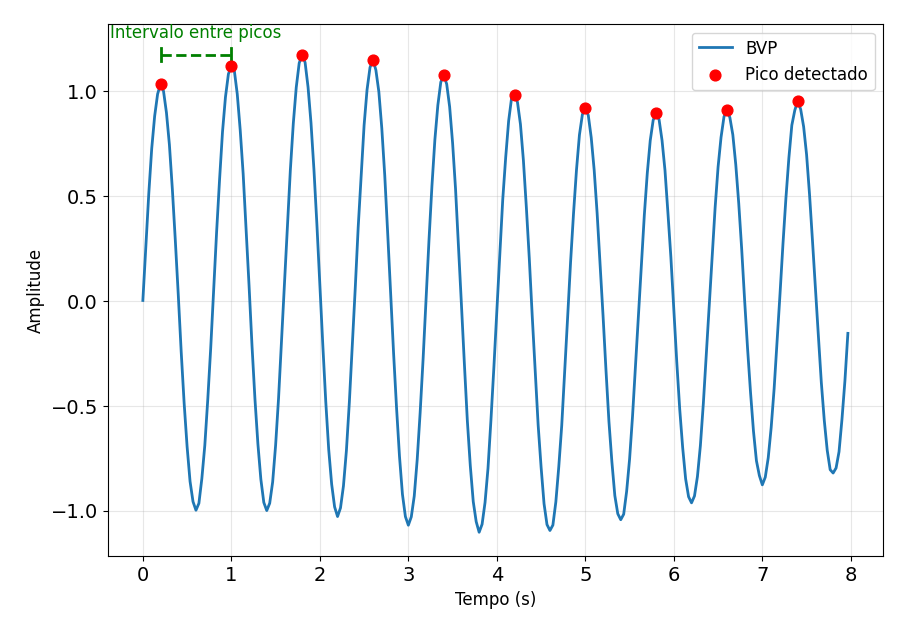
\includegraphics[width=\linewidth]{imagens/dominio_tempo.png}
\caption{}
\label{fig:fc_tempo}
\end{subfigure}
\hfill
\begin{subfigure}{0.45\textwidth}
\centering
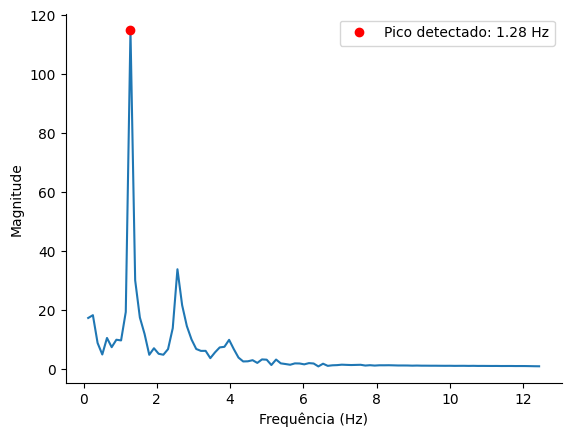
\includegraphics[width=\linewidth]{imagens/dominio_freq.png}
\caption{}
\label{fig:fc_freq}
\end{subfigure}

\caption{Representação de técnicas de estimativa da frequência cardíaca no domínio do tempo (a) e no domínio da frequência (b). No domínio do tempo, os picos do sinal de rPPG são detectados e, a partir da média de intervalo entre picos, a frequência cardíaca é estimada. No domínio da frequência, a estimativa de FC é realizada por meio da identificação do primeiro pico mais proeminente no espectro da série temporal do sinal de rPPG, correspondente à frequência fundamental.}
Fonte: autoria própria
\label{fig:det_freq_card}
\end{figure}

% Citar métodos supervisionados para extração da frequência cardíaca \cite{vspetlik2018visual}

\subsection{Variabilidade da frequência cardíaca}

A variabilidade da frequência cardíaca (HRV) refere-se à variação do intervalo de tempo entre batimentos cardíacos consecutivos e permite a avaliação da saúde do sistema cardíaco, especialmente do funcionamento do sistema nervoso autônomo responsável por sua regulação \cite{acharya2006heart}. Esse parâmetro é comumente calculado com base no eletrocardiograma, no entanto pode ser estimado de maneira consistente pela variabilidade da frequência de pulso baseada na onda de PPG para indivíduos em repouso \cite{schafer2013accurate}. Para isso, analisa-se a variação dos intervalos entre picos ao longo do tempo da onda de pulso de volume sanguíneo. 

No contexto da fotopletismografia remota, é demonstrado que a estimativa da frequência cardíaca pode ser obtida com acurácia satisfatória por meio da identificação da frequência predominante do espectro do sinal obtido por câmera. Todavia, a identificação dos intervalos entre batimentos ainda apresenta-se como um desafio. Isso ocorre devido sobretudo à necessidade da detecção precisa de picos do sinal, a qual requer uma relação sinal-ruído adequada que normalmente não é obtida pela medição remota, e devido à necessidade de uma frequência de amostragem mínima para a obtenção de valores de HRV confiáveis, especificamente de 100 Hz no caso da obtenção a partir do eletrocardiograma \cite{malik1996heart}. No caso da obtenção a partir do sinal de PPG, é possível verificar que a obtenção de medidas de HRV tanto no domínio do tempo quanto no domínio da frequência a partir do sinal de fotopletismografia amostrado a 1000 Hz pode ser comparável a medidas obtidas a partir do sinal amostrado a 50 Hz \cite{pelaez2021impact}, valor que, no entanto, não é comumente atingido por câmeras convencionais.

Apesar disso, é possível demonstrar que a interpolação do sinal de rPPG obtido com taxas de quadros menores do que a necessária gera resultados de estimativa de variabilidade da frequência cardíaca próximos aos obtidos com a taxa mínima e com boa correlação quando comparados aos obtidos por sensores de contato \cite{sun2013noncontact}. Ademais, estratégias de otimização da detecção dos picos da onda de BVP medida remotamente contribuem para a obtenção de valores do intervalo entre picos com boa correlação em relação aos valores de referência \cite{maki2019inter, li2020video}. Analogamente, soluções de aprendizado profundo focadas na redução do ruído dos sinais de crominância capturados por câmera para geração de formas de onda de BVP realistas permitem a otimização da acurácia da estimativa do intervalo entre pulsos e, consequentemente dos parâmetros relacionados à variabilidade de frequência cardíaca  \cite{Song2021pulsegan, yang2023cbppggan}. 

\subsection{Frequência respiratória}

A onda de fotopletismografia reflete a pulsação cardiogênica ao representar as variações temporais no volume sanguíneo periférico, decorrentes da propagação da onda de pulso ao longo do ciclo cardíaco. No entanto, o sinal fotopletismográfico também é influenciado pelo sistema respiratório, de forma que a onda de pulso de volume sanguíneo característica da fotopletismografia também é modulada por três principais fatores relacionados à respiração, conforme exibido na \autoref{fig:resp-mods}. Primeiramente, há uma modulação da linha de base do sinal, induzida pelo retorno venoso causado pelas mudanças na pressão intratorácica que acontecem durante a inspiração e a expiração. Além disso, essas mudanças de pressão resultam em variações do volume de sangue expelido pelo ventrículo esquerdo, o que gera uma modulação de amplitude da onda. Por fim, há uma modulação da frequência do sinal de PPG gerada pela variação da frequência cardíaca ao longo do ciclo respiratório, em que há a redução do período cardíaco durante a inspiração e um aumento ao longo da expiração devido à atuação do sistema nervoso autônomo, fenômeno denominado arritmia sinusal respiratória. Assim, os efeitos desses fatores podem ser identificados, o que faz com que seja possível extrair informações da respiração pela onda característica de PPG com o uso de algoritmos os quais também podem ser aplicados ao sinal obtido remotamente \cite{luguern2020assessment}. 

\begin{figure}[h!]
    \centering
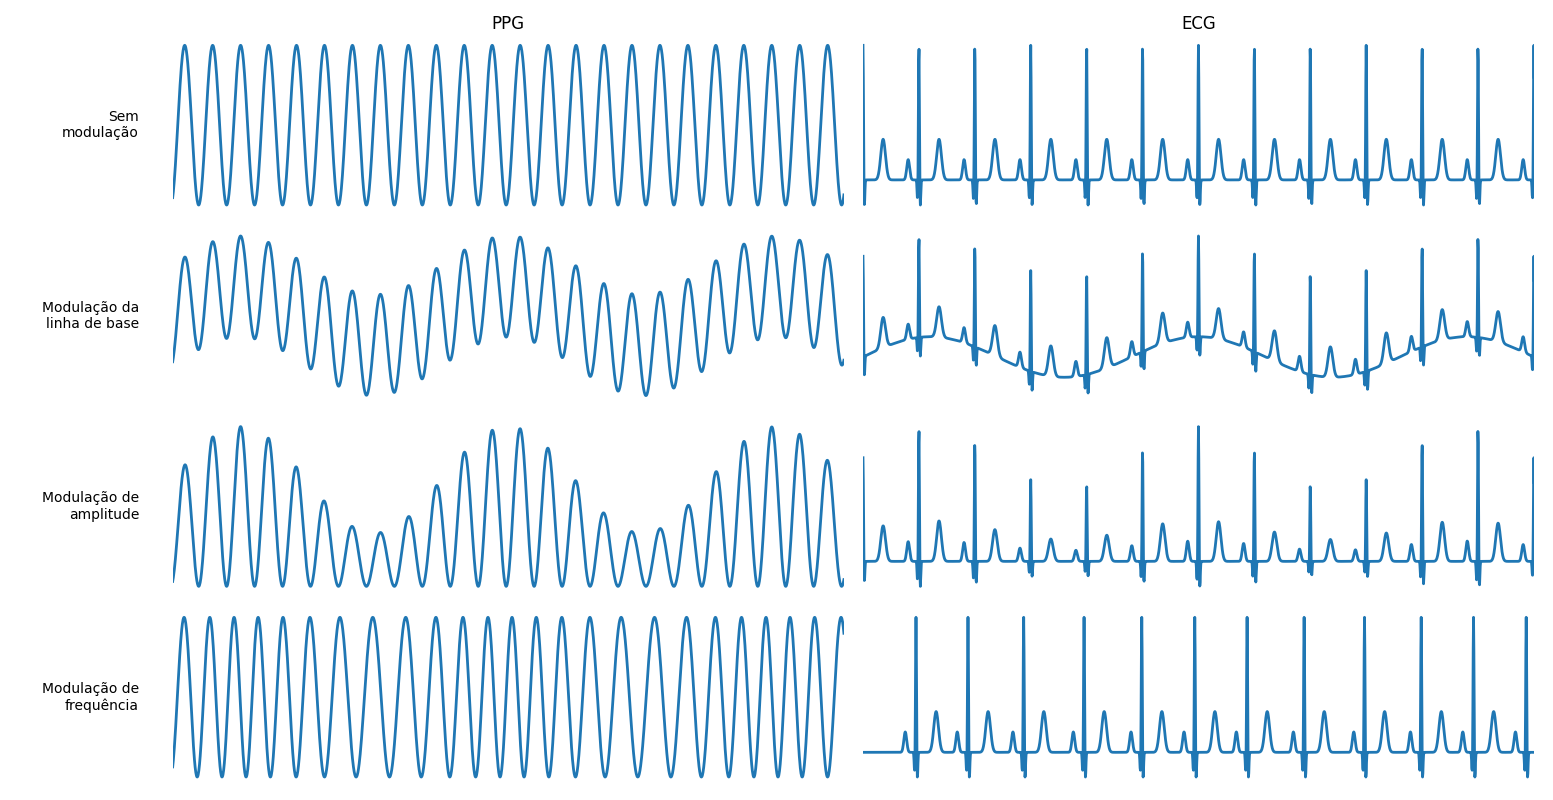
\includegraphics[width=\linewidth]{imagens/resp_mods.png}
    \caption{Exemplos das modulações respiratórias observadas em sinais de fotopletismografia (PPG) e eletrocardiografia (ECG). A primeira linha apresenta os sinais sem influência respiratória. As linhas subsequentes ilustram, respectivamente, a modulação da linha de base, caracterizada pelo deslocamento periódico do nível médio do sinal; a modulação de amplitude, associada a variações na amplitude dos picos; e a modulação de frequência, relacionada às alterações cíclicas no espaçamento entre picos consecutivos do sinal.}
    Fonte: Adaptado de \citeonline{charlton2016assessment}
    \label{fig:resp-mods}
\end{figure}

No contexto do monitoramento por câmera, duas das principais abordagens envolvem detectar as modulações induzidas pelo ciclo respiratório no sinal de rPPG ou detectar as variações induzidas pelo movimento causado pela respiração \cite{wei2017non, schrumpf2019exploiting}, sendo que a primeira atinge melhor acurácia e apresenta maior confiabilidade \cite{boccignone2023evaluation}. De fato, é possível demonstrar que essas modulações podem ser identificadas pela análise das variabilidades da largura, da frequência e da amplitude de pulso \cite{iozzia2017respiratory}. Mais recentemente, soluções de aprendizado profundo permitem a obtenção de sinais cardíaco e respiratório a partir de modelos multi-tarefas \cite{lee2022multitask, liu2020multi}. 

\subsection{Saturação periférica de oxigênio (SpO2)}

A saturação periférica de oxigênio (SpO2) corresponde à razão entre as concentrações da hemoglobina oxigenada e da hemoglobina total presente no sangue, sendo que há diferenças significativas entre a absorção de luz pela oxihemoglobina e pela desoxihemoblobina ao longo dos diversos comprimentos de onda, de forma proporcional às respectivas concentrações. Assim, a fotopletismografia permite a identificação desse parâmetro por meio da análise da razão entre as amplitudes da componente AC do sinal sob iluminações referentes ao vermelho e ao infravermelho próximo, bem como da componente DC correspondente. A escolha desses comprimentos de onda se dá devido à diferença de absorção das duas substâncias, o que faz com a comparação seja sensível a mudanças na oxigenação \cite{allen2007photoplethysmography}. 

Diferente da medição por contato, a estimativa da SpO2 a partir do sinal obtido remotamente deve levar em consideração a região do espectro luminoso capaz de ser capturada pelo sensor óptico da câmera sob iluminação ambiente. Nesse sentido, as soluções nesse contexto utilizam a comparação entre o vermelho e o verde, considerando as diferenças de absorção pela oxihemoglobina e pela desoxihemoglobina nesses comprimentos de onda \cite{kong2013non}, apesar de a profundidade atingida no tecido cutâneo ser menor na faixa do verde, quando comparada ao infravermelho próximo e ao vermelho \cite{mocco2021pulse}. Outras implementações demonstram, ainda, que a utilização dos sinais dos canais azul e vermelho gera resultados comparáveis aos obtidos por um oxímetro de pulso \cite{casalino2020mhealth, gs2024remote, guazzi2015non}.

\subsection{Pressão arterial}

A pressão sanguínea refere-se à força que o sangue exerce contra as paredes dos vasos sanguíneos enquanto circula pelo sistema cardiovascular. Esse parâmetro é frequentemente medido de forma invasiva por cateterismo ou de forma não invasiva por ausculta ou método oscilométrico com a utilização de manguitos pressurizados. No entanto, há soluções que estimam esse sinal a partir do tempo de trânsito de onda de pulso (\textit{Pulse Transit Time} - PTT), o qual corresponde ao tempo que a onda de pressão leva para percorrer duas regiões diferentes do sistema arterial. No contexto da fotopletismografia, a medição do PTT pode ser realizada por meio da comparação dos sinais de dois oxímetros medidos em locais distintos \cite{mukkamala2015toward}. 

No cenário do monitoramento remoto, por sua vez, o tempo de trânsito de onda de pulso  pode ser obtido a partir de duas medições remotas realizadas em locais diferentes, como na região do pé e da mão \cite{murakami2015non} ou na região do rosto em comparação com a palma da mão \cite{fan2020robust}. Por fim, a partir do PTT, a pressão sanguínea é estimada por meio de estratégias de calibração. Outras soluções aproximam esse parâmetro pelo tempo de chegada de pulso (\textit{Pulse Arrival Time} - PAT) estimado como o tempo entre o pico R do ECG e o pé do sinal de rPPG extraído do rosto \cite{secerbegovic2016blood}.

Soluções mais recentes, por outro lado, permitem a estimativa da pressão sanguínea remotamente com base na análise unicamente da região do rosto. Para isso, são implementadas estratégias de aprendizado de máquina, por exemplo, para relacionar esse parâmetro com a distribuição espacial e temporal do sinal de pulso facial utilizando modelos de redes neurais convolucionais \cite{iuchi2022blood} ou uma combinação desse tipo de modelo para extrair características espaciais com redes neurais recorrentes para análise temporal \cite{hamoud2023neural}. É possível, ainda, relacionar a pressão sanguínea com o sinal de rPPG e outros indicadores fisiológicos, como a frequência cardíaca e o tempo de trânsito da onda de pulso, com o uso de redes neurais profundas \cite{wu2022facial}.


% \subsection{Perfusão sanguínea periférica}